\documentclass[../../notes.tex]{subfiles}

\pagestyle{main}
\renewcommand{\chaptermark}[1]{\markboth{\chaptername\ \thechapter\ (#1)}{}}
\setcounter{chapter}{3}

\begin{document}




\chapter{Continuity}
\section{Notes}
\begin{itemize}
    \item \marginnote{11/8:}Consider a function $f:X\to Y$ whose domain and codomain are, respectively, the metric spaces $(X,d_X)$ and $(Y,d_Y)$.
    \item \textbf{Limit} (of $f$ at $p$): A point $q\in Y$ such that for all $\epsilon>0$, there exists $\delta$ such that $d_X(x,p)<\delta$ implies $d_Y(q,f(x))<\epsilon$, where $p$ is a limit point of $X$ (otherwise, $x\nrightarrow p$).
    \item \textbf{Continuous} (function $f$ at $p$): A function $f$ such that $\lim_{x\to p}f(x)=f(p)$.
    \item $f$ is continuous on $X$ if it is continuous at every $p\in X$.
    \item \textbf{Uniformly continuous} (function $f$): A function $f$ such that for every $\epsilon>0$, there exists a $\delta>0$ such that $d_X(x,y)<\delta$ implies $d_Y(f(x),f(y))<\epsilon$ for all $x,y\in X$.
    \item \marginnote{11/10:}$f,g$ continuous implies $f+g$, $fg$, and $f/g$ continuous, the latter where $g(x)\neq 0$.
    \item If $f,g$ continuous, then $h=g\circ f$ is continuous.
    \item Theorem: $f:X\to Y$ is continuous iff $f^{-1}(V)$ is open in $X$ for every $V\subset Y$ open.
    \begin{figure}[h!]
        \centering
        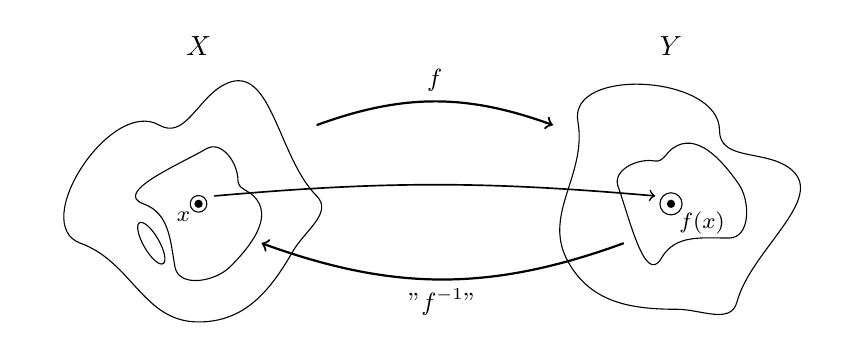
\begin{tikzpicture}
            \footnotesize
            \fill circle (1.5pt) node[below left]{$x$};
            \draw circle (3pt);
            \draw (0.1,0.7)
                to[out=30,in=90] (0.5,0.3)
                to[out=-90,in=135] (0.7,0.1)
                to[out=-45,in=45] (0.4,-0.8)
                to[out=-135,in=-80] (-0.3,-0.8)
                to[out=100,in=-20] (-0.7,0)
                to[out=160,in=-150] cycle
            ;
            \draw [rotate around={-60:(-0.6,-0.5)}] (-0.6,-0.5) ellipse (3mm and 1mm);
            \draw (0.3,1.5)
                to[out=30,in=135] (1.5,0.1)
                to[out=-45,in=60] (1.2,-0.6)
                to[out=-120,in=0] (0,-1.5)
                to[out=180,in=-20] (-1.5,-0.5)
                to[out=160,in=150] (-0.5,1)
                to[out=-30,in=-150] cycle
            ;
    
            \begin{scope}[xshift=6cm]
                \fill circle (1.5pt) node[below right]{$f(x)$};
                \draw circle (4pt);
    
                \draw [rotate=80] (0.1,0.7)
                    to[out=30,in=90] (0.5,0.3)
                    to[out=-90,in=135] (0.7,0.1)
                    to[out=-45,in=45] (0.4,-0.8)
                    to[out=-135,in=-80] (-0.3,-0.8)
                    to[out=100,in=-20] (-0.7,0)
                    to[out=160,in=-150] cycle
                ;
                \draw [rotate=-60] (0.3,1.5)
                    to[out=30,in=135] (1.5,0.1)
                    to[out=-45,in=60] (1.2,-0.6)
                    to[out=-120,in=0] (0,-1.5)
                    to[out=180,in=-20] (-1.5,-0.5)
                    to[out=160,in=150] (-0.5,1)
                    to[out=-30,in=-150] cycle
                ;
            \end{scope}
    
            \normalsize
            \node at (0,2) {$X$};
            \node at (6,2) {$Y$};
    
            \small
            \draw [thick,->] (1.5,1) to[bend left=20] node[above]{$f$} (4.5,1);
            \draw [semithick,->] (0.2,0.1) to[bend left=5] (5.8,0.1);
            \draw [thick,->] (5.4,-0.5) to[bend left=20] node[below]{"$f^{-1}$"} (0.8,-0.5);
        \end{tikzpicture}
        \caption{Set theoretic definition of continuity.}
        \label{fig:continuityOpenSets}
    \end{figure}
    \begin{itemize}
        \item This works in a general topological space, too, not just a metric space.
        \item Note that $f^{-1}(V)$ is not a function defined on $V$; it's a specifically defined set $\{x\in X:f(x)\in V\}$.
        \item $f$ being continuous means that open circular neighborhood of a point $x$ in the domain maps to an area of the range encompassed by a circular neighborhood of $f(x)$.
        \item The other condition means that every open set surrounding $f(x)$ maps to an open set of the domain surrounding $x$. Indeed, going off of this definition, if an open set containing $f(x)$ maps to an open set containing $x$, then we can choose a neighborhood subset of the open set surrounding $x$ and know that it will map into a neighborhood subset of the open set surrounding $f(x)$. 
    \end{itemize}
    \item Corollary: $f:X\to Y$ continuous iff $f^{-1}(C)$ closed for every $C\subset Y$ closed.
    \begin{itemize}
        \item We use the property that $f^{-1}(X\subset C)=X\subset f^{-1}(C)$.
    \end{itemize}
    \item Let $f_1:X_1\to Y_1$ and $f_2:X_2\to Y_2$. Suppose $f:X_1\times X_2\to Y_1\times Y_2$ is defined by $f(x_1,x_2)=(f_1(x_1),f_2(x_2))$. Then $f$ is continuous iff $f_1,f_2$ are continuous, under appropriately defined metrics.
    \item Continuity and compactness.
    \item Theorem: $f:X\to Y$ continuous and $X$ compact imply $f(X)$ compact.
    \begin{itemize}
        \item Let $\{V_\alpha\}$ be an open cover of $f(X)$.
        \item Then $\{f^{-1}(V_\alpha)\}$ is an open cover of $X$..
        \item Choose a finite subcover of $\{f^{-1}(V_\alpha)\}$. Then the corresponding $V_\alpha$'s form a finite subcover of $f(X)$.
    \end{itemize}
    \item If $f:X\to\R^k$ is continuous and $X$ is compact, $f(X)$ is compact and closed/bounded.
    \item If $f:X\to\R$ is continuous and $X$ is compact, then $M=\sup_{x\in X}|f(x)|=|f(\bar{x})|$ and $m=\inf{x\in X}|f(x)|=|f(\underline{x})|$ where $\bar{x},\underline{x}\in X$.
    \begin{itemize}
        \item There is a subsequence $\{x_m\}$ such that $|f(x_m)|\to M$. Since $f(X)$ is compact, the limit of this sequence is in $f(X)$.
    \end{itemize}
    \item If $f:X\to Y$ is continuous, bijective, and $X,Y$ are compact, $f^{-1}:Y\to X$ is continuous.
    \item Uniform continuity.
    \item Examples.
    \begin{itemize}
        \item Linear functions are uniformly continuous.
        \item $f:(0,1)\to\R$ defined by $f(x)=x^2$ is uniformly continuous.
        \item $f:(a,\infty)\to\R$ defined by $f(x)=x^2$ is \emph{not} uniformly continuous.
        \item $f:(a,\infty)\to\R$ defined by $f(x)=1/x$ is uniformly continuous if $a>0$.
        \item $f:(0,\infty)\to\R$ defined by $f(x)=1/x$ is \emph{not} uniformly continuous.
    \end{itemize}
    \item \textbf{Lipschitz continuous} (function $f$ on $E\subset X$): A function such that $|f(x)-f(y)|\leq L|x-y|$ for each $x,y\in E$.
    \item Theorem: $f:X\to Y$ continuous and $X$ compact implies $f$ is uniformly continuous.
    \begin{itemize}
        \item Fix $\epsilon>0$. There exists $\delta=\delta(p)>0$.
        \item Def. of continuity: $q\in N_{\delta(p)}(p)$ implies $f(q)\in N_\epsilon(f(p))$.
        \item $\{N_{\delta(p)/2}(p):p\in X\}$ is an open cover of $X$. Choose a finite subcover. Let $\delta=\min(\delta(p_1)/2,\dots,\delta(p_n)/2)$.
        \item ...
    \end{itemize}
    \item \marginnote{11/12:}$f:X\to Y$ continuous and $E\subset X$ connected implies $f(E)$ connected.
    \begin{itemize}
        \item Suppose $f(E)=A\cup B$, $A,B$ nonempty, separated subsets of $Y$.
        \item Let $G=E\cap f^{-1}(A)$, $H=E\cap f^{-1}(B)$. It follows that $E=G\cup H$, where $G,H$ nonempty.
        \item $A\subset\bar{A}$ implies $G\subset f^{-1}(\bar{A})$ implies (inverse image def. of continuity) $\bar{G}\subset f^{-1}(A)$ implies $f(\bar{G})\subset \bar{A}$.
        \item $f(H)=B$ and $\bar{A}\cap B=\emptyset$ yields $\bar{G}\cap H=\emptyset$. Symmetrically, $G\cap\bar{H}=\emptyset$. This contradicts our assumption that $E$ is connected.
    \end{itemize}
    \item Introduces monotone functions.
    \item Theorem: If $f$ is monotonic on $(a,b)$, then the set of points of $(a,b)$ at which $f$ is discontinuous is at most countable.
    \begin{itemize}
        \item ...
    \end{itemize}
\end{itemize}



\section{Chapter 4: Continuity}
\emph{From \textcite{bib:Rudin}.}
\begin{itemize}
    \item \marginnote{11/8:}\textbf{Limit} (of $f$ at $p$): The point $q\in Y$, if it exists, such that for every $\epsilon>0$, there exists a $\delta>0$ such that $d_Y(f(x),q)<\epsilon$ for all points $x\in E$ for which $0<d_X(x,p)<\delta$, where $(X,d_X),(Y,d_Y)$ are metric spaces, $E\subset X$, $f:E\to Y$, and $p\in E'$. \emph{Denoted by} $\bm{\lim_{x\to p}f(x)}$.
    \begin{itemize}
        \item Note that we do not require that $p\in E$; only that some elements of the domain $E$ approach $p$.
        \item We also write $f(x)\to q$ as $x\to p$.
    \end{itemize}
    \item Theorem 4.2: Let $X$, $Y$, $E$, $f$, and $p$ be as specified above. Then $\lim_{x\to p}f(x)=q$ iff $\lim_{n\to\infty}f(p_n)=q$ for every sequence $\{p_n\}$ in $E$ such that $p_n\neq p$ for any $n$ and $\lim_{n\to\infty}p_n=p$.
    \item \textcite{bib:Rudin} proves the sum, product, and quotient rules of limits from the analogous properties of series.
    \item Continuity is defined.
    \begin{itemize}
        \item Note that $f$ \emph{does} have to be defined at $p$ to be continuous at $p$ (in comparison to the fact that it can have a limit at a point $p'$ at which it is not defined).
        \begin{itemize}
            \item Thus, for proofs concerning continuity (as opposed to limits), we will consider functions $f$ the domains of which are metric spaces, not \emph{subsets} of metric spaces.
        \end{itemize}
        \item It follows from the definition that if $p\in E$ is isolated, then every possible $f$ defined on $E$ is continuous at $p$.
    \end{itemize}
    \item Theorem 4.7: Compositions of continuous functions are continuous.
    \item Theorem 4.8: Preimage definition of continuity.
    \item Theorem 4.9: If $f,g$ are complex continuous functions on $X$, $f+g$, $fg$, and $f/g$ are continuous on $X$.
    \item Theorem 4.10: $\fb$ continuous implies $f_1,\dots,f_k$ continuous. Also, $\fb,\gb:X\to\R^k$ continuous implies $\fb+\gb$ and $\fb\cdot\gb$ continuous.
    \item \marginnote{11/9:}Theorem 4.14: $f$ continuous and $X$ compact implies $f(X)$ compact.
    \item Theorem 4.15: $\fb:X\to\R^k$ continuous and $X$ compact implies $f(X)$ closed and bounded.
    \item Theorem 4.16: $f$ continuous and $X$ compact implies $f$ attains its minimum and maximum.
    \item Theorem 4.17: $f:X\to Y$ continuous, 1-1 for $X,Y$ compact implies $f^{-1}:Y\to X$ continuous.
    \item Theorem 4.19: $f$ continuous and $X$ compact implies $f$ uniformly continuous.
    \item Theorem 4.20: Compactness is a necessary condition in Theorems 4.14, 4.15, 4.16, and 4.19.
    \item Theorem 4.22: $f:X\to Y$ continuous and $E\subset X$ connected implies $f(E)$ connected.
    \item Theorem 4.23: Intermediate value theorem.
    \item \textbf{Right-hand limit} (of $f$ at $x$): \emph{Denoted by} $\bm{f(x+)}$.
    \item \textbf{Left-hand limit} (of $f$ at $x$): \emph{Denoted by} $\bm{f(x-)}$.
    \item \textbf{Discontinuity of the first kind} (of $f$ at $x$): A discontinuity of $f$ at $x$ such that $f(x+)$ and $f(x-)$ exist. \emph{Also known as} \textbf{simple discontinuity}.
    \item \textbf{Discontinuity of the second kind} (of $f$ at $x$): A discontinuity of $f$ at $x$ that is not of the first kind (i.e., a discontinuity such that at least one of $f(x+)$ and $f(x-)$ does not exist).
    \item Theorem 4.29: If $f$ is monotonic on $(a,b)$, then $f(x+),f(x-)$ exist at every $x\in(a,b)$.
    \item Corollary: Monotonic functions have no discontinuities of the second kind.
    \item Theorem 4.30: If $f$ is monotonic on $(a,b)$, then the set of points of $(a,b)$ at which $f$ is discontinuous is at most countable.
\end{itemize}




\end{document}